\chapter{Rastreamento Ocular}

\section{Anatomia Ocular}
O globo ocular é majoritariamente opaco, com exceção da córnea, que é transparente. 
A pupila é a região que da passagem para a luz e possui diâmetro variável. Os músculos da íris são os que controlam a dilatação da pupila. 
A focalização da imagem deve se concentrar na fóvea, onde se encontram células muito sensíveis a luz (Helene e Helene, 2011). 
A fixação ocular compreende a um período de cerca de 100 milissegundos onde o olhar se fixa em um ponto de convergência (Barreto et al., 2012). 
Este período se encerra com o movimento de sacada, que compreende ao movimento rápido até uma nova fixação do olhar em outro local.
Através da coleta do posicionamento ocular, é possível calcular uma taxa de dispersão focal ao longo do tempo e piscadas. 
Estes dados foram previamente correlacionados com estados emocionais (Soleymani et al., 2012) e 
também aplicados em estudos com algoritmos de aprendizado de máquina e deep learning. Barreto (2012)
resumiu alguns dos principais termos utilizados em pesquisas de rastreamento ocular (RO):

\begin{figure}[h]
    \centering
    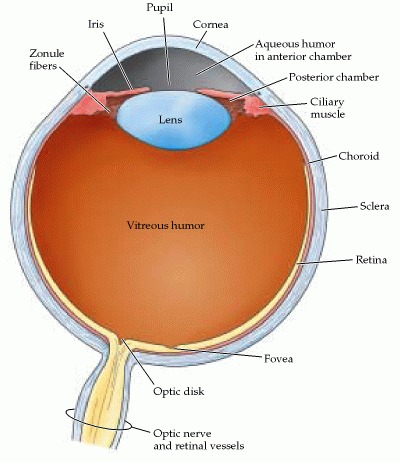
\includegraphics[width=100mm]{anatomy.jpeg}
    \caption[]{}\label{fig:}
    \end{figure}

\section{Equipamentos de Rastreamento}
Para detectar onde o participante está focando seu olhar ao longo do tempo, alguns equipamentos de ET
 fazem uso de luz infravermelha e câmeras de alta definição que projetam a luz
  diretamente no olho do participante e gravam a direção do olhar a partir do reflexo. 
  Como a luz infravermelha abrange um comprimento de onda não detectável pelo olho humano, 
  o direcionamento desta luz no olho não interfere visão do participante. 
  O cálculo do direcionamento ocular é feito com base em algoritmos próprios de cada fabricante. 
  Existem alguns tipos de equipamentos de rastreamento ocular. São eles: (1) Webcam, (2) Vestível (Werable) e (3) Baseados em Tela. 
  Webcam diz respeito a equipamentos não especializados para o uso de rastreamento; usáveis correspondem a equipamentos como óculos de rastreamento ocular 
  e realidade virtual, e os baseados em tela dizem respeito aos equipamentos de coleta especializada que podem ser acoplados a um computador Tobii Pro (2020).
